\section{Introduction}

\label{sec:intro}

% ==================First Paragraph================================== 
% Current approach is driven by existed dataset

% IM2GPS Hays08								Hays08
% Tiny Image									Torralba08
% Mapping the World's Photo		Crandall09  Flickr
% SUN attribute								Xiao10
% Location recognition using prioritized feature matching								Li2010				Cornell dataset

% City-Scale Location Recognition																				Schindler07
% Accurate Image Localization Based on Google Maps Street View					RoshanZamir10

Image based geolocation draws the attention from computer vision society in the past few years.  The massive collections of publicly available imagery is the key to enable location recognition.  \cite{Hays08}, \cite{Torralba08}, \cite{Li10}, \cite{Crandall09}, \cite{Xiao10}, \cite{Li10} harvest millions of geotagged images from photo sharing website.  \cite{Schindler07}, \cite{RoshanZamir10} also collect millions of images from the street view services along tens to hundreds kilometer of the street side.  With the large image database, the exciting progress has been made by applying popular object recognition techniques at two ends of the spectrum: holistic image-as-texture based matching (e.g., “the photo depicts an Iberian scene”) and local interest point based near-duplicate retrieval for famous landmarks (e.g., “the photo depicts the Sagrada Família”).  One common property shared by the both methods is that the query image should be taken \emph{within-condition} as the images in database for successful retrieval.

%1. image based geolocation draws attention from Computer Vision society in past few years.
%2. The key reason to enable the proliferation of field is the large image data set
%3. Variety of public available geotagged images on the Internet. photo sharing websites, Google Street View services
%4. The exciting progress has been made by the method inspired by previous data with near duplicate image retreival method.  (popular landmark)
%5. One common property shared by the previous methods is that near duplicate approach can produce good result for matching image within the same condition.

% ==================Second Paragraph==================================
% Introduce the dataset: setting, why do we need this kind of techniques, challenge, expected result
% The hope and the future work of GLAID

On the contrary of the popularity of matching images from photo sharing websites and street view services, the $45^\circ$ aerial imagery receives less attention in the wave of data driven location recognition despite the aerial imagery database has the mertis of wide and uniform coverage of locations, easy availability, and accurate geotagged images.  The above metioned merits could potentially complement the existed databases which put more emphasis on matching popular landmarks or street images.  However, the mismatch of disparity of view and imaging conditions between the query image and image database might arise the new challengings for matching holistic features or finding the near-duplicate local descriptor.  Such \emph{cross-condition} image matching still mainly untouched and needs a systematic study to discover the performance limit with the existed methods.


%0. point out the aerial database receive less attention
%1. But aerial imagery has the advantages such as wide and uniform coverage, xxxx that could complement existed datasets.
%2. The new challenge the mismatch of disparity of view and imaging conditions could make near duplicate feature matching failure therefore making the problem extremely challenging
%3. It's unknown about how good the existed data driven approach can acheive when applying on GLAID


% ==================Third Paragraph==================================
We introduce GLAID that aims to match ground level image to $45^\circ$ aerial imagery database. We benchmark top-down holistic image-as-texture based matching and bottom-up local interest point near-duplicate retrieval, providing an overview of the performance for the new challenge.  We propose a new performance metric based on the ranking of correct location at the set of blockified aerial images.  We label the affine transoformation and point correspondences between of each query image to the aerial imagery database such that we can study the variation of the distance for the corresponded pair of local feature descriptors.  We hope that the experiment result of baseline benchmark can shed the light on the future research directions for ground level to aerial level mathcing or more general \emph{cross condition} image matching.
 
% 1. We introduce GLAID that aims to match query image to $45^\circ$ aerial imagery.
% 2. some feature of the dataset, the location and affine transformation
% 3. we benchmark the dataset
% 4. A new performance metric is introduced to genuine location.
% 5. we hope the experiement result can indentify the directions of research for cross condition matching

% ==================Fourth Paragraph==================================
This paper is organized as follow.  The next section reviews top-down and bottom-up approaches for geolocation in the related works.  Section \ref{sec:image} introduces the image collection and annotation of GLAID dataset.  The baseline experiment settings and the experiment result are shown in Section \ref{sec:experiment} and Section \ref{sec:result}.  Finally, we will analyze the common failure cases of the baseline approach and identify the future direction for cross condition ground level to aerial image matching.  

% Content and emphasis for each section
%1. in section 2, we discuss the two popular approches that are usually used for geolocation
%2. in section 3, we introduce the details of image dataset
%3. in section 4, we discuss the detail approach of our baseline experiment
%4. in section 4, we show the baseline experiment result
%5. in section 5, we discuss the failure case and the future work

%Local:
%Location Recognition using prioritized feature matching
%- P2F: set the number of uniquely matched feature to be N
%Accurate Image Localization Based on Google Maps Street View
%- voting
%City-Scale Location Recognition
%- vocabulary tree on SIFT

%The problem of geographically localizing an image presents a wide array of challenges in computer vision and machine learning.  To answer the question ``where was this photo taken?''~when GPS data is not available, one can appeal to a variety of publicly available geotagged images on the Internet, e.g., photo sharing websites, street view services, satellite and aerial imagery. The problem of matching and retrieving images captured \emph{within-condition} using nearest neighbor on semi-local descriptors is well studied.  The same problem is considerably more difficult for the case of cross-condition image matching, e.g., in which there are significant differences in the noise level, blur, or illumination between a given pair of images; see Fig.~\ref{dataset-b}. The mismatch of features can severely degrade the accuracy of nearest neighbor methods. A solution to the problem of cross-condition matching is therefore key to leveraging the vast and diverse array of geotagged image data available on the Internet.

%To address this problem, we propose a human-in-the-loop, active learning framework. We leverage the relative ease with which a human observer can establish correspondences between categorically similar local image regions corresponding to meaningful architectural or landscape primitives such as window pane, chimney or shrub. First, the user is asked to select a few distinctive regions of interest in the query (ground level) image. Then the user is asked to label some patches with similar or dissimilar appearance in the aerial image.  Given this data, we learn a metric space wherein the extracted features from the two images are directly comparable.  To reduce the human labeling effort and improve the accuracy of the computer vision method, the proposed system alternates between computer vision processing and requesting user feedback. During this process, the system intelligently selects the instances with highest expected information gain for labeling. This active learning framework iteratively improves the metric, thereby allowing the system to find the genuine location with reduced human effort.

%This paper is organized as follows. The next section reviews related work.  Section \ref{sec:hil} reviews the proposed human-in-the-loop system. Then the learning algorithm will be explained in Section \ref{sec:learning}. Sections \ref{sec:dataset}, \ref{sec:feature} and \ref{sec:exper} explain the GLAID dataset, feature extraction and matching, and experimental results respectively. Finally, we conclude in Section \ref{sec:concl}. 

\begin{figure}[t] 
\centering
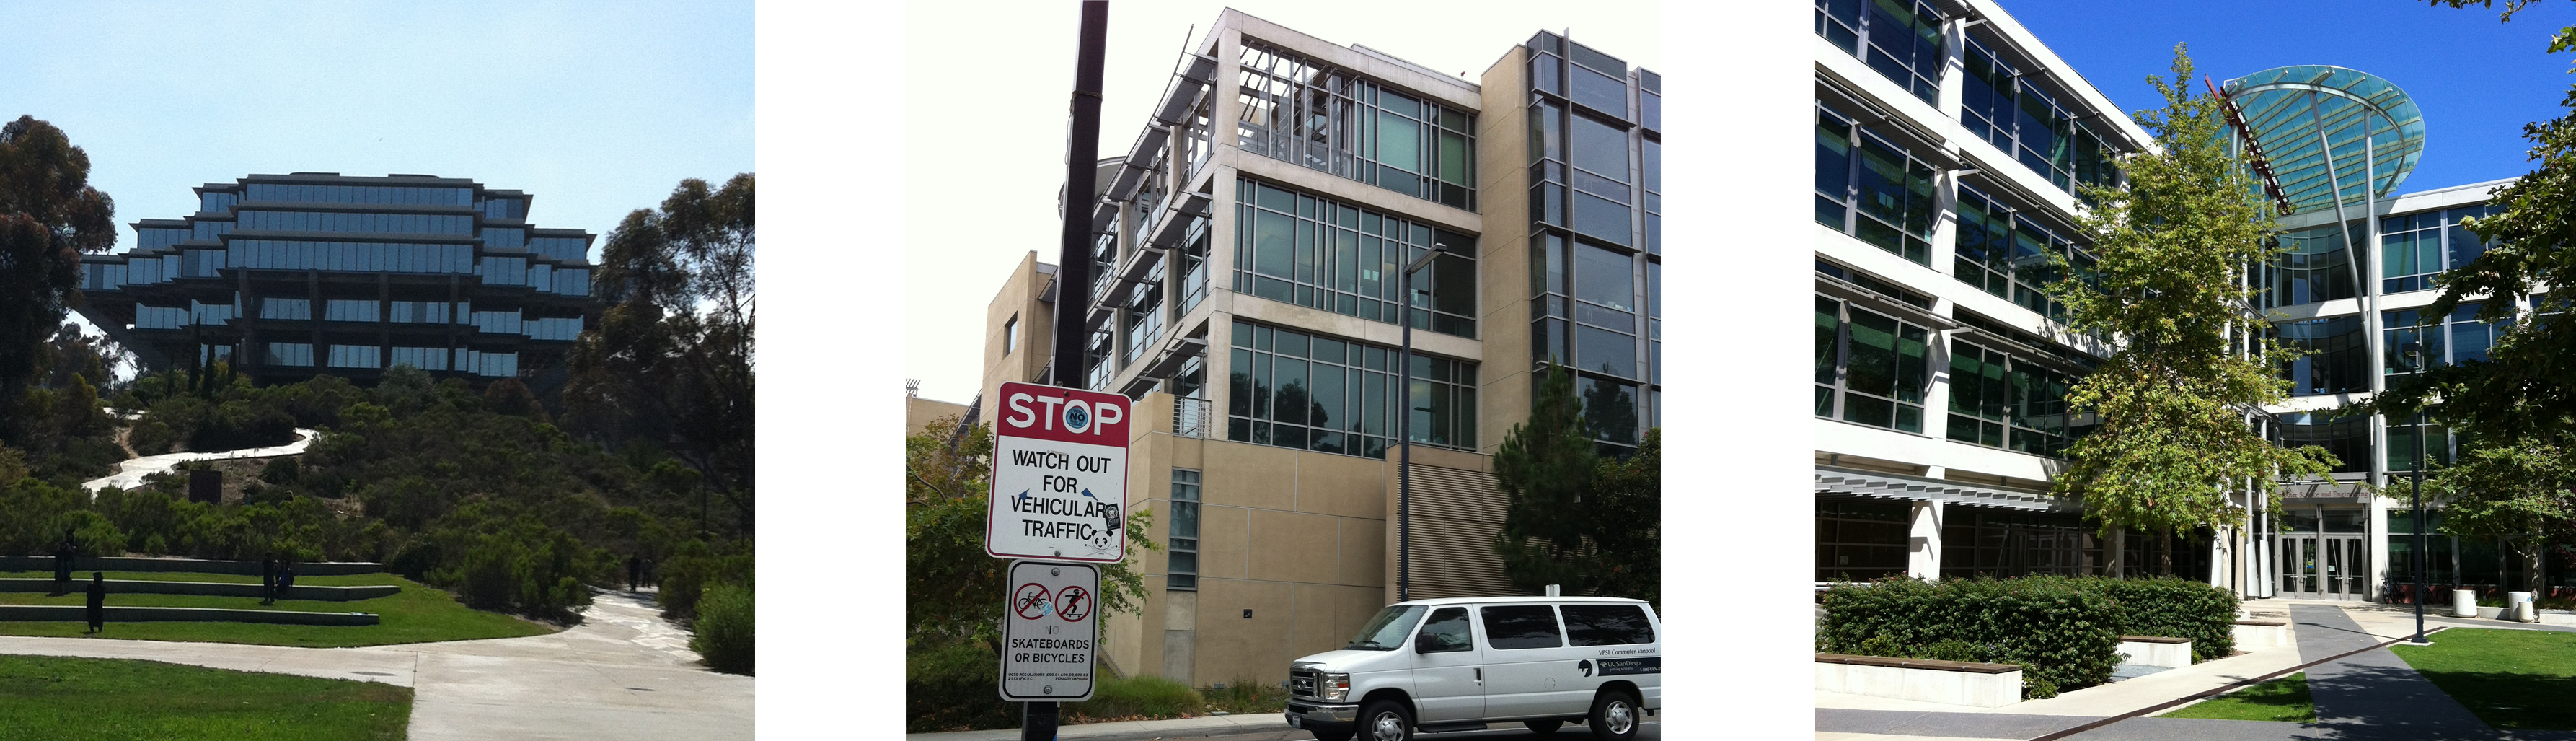
\includegraphics[width=0.9\textwidth]{pictures/exampleImg} \label{example} }
\caption[]{Snapshot of GUI for relevance feedback from the user.}
\label{fig:exampleImg}
\end{figure}

